\documentclass{article}      % Specifies the document class

% -------------------- Packages --------------------
\usepackage{amsmath}
\usepackage{amssymb}
\usepackage[noend]{algpseudocode}
\usepackage{algorithm}
\usepackage{graphicx}
\usepackage{float}
\usepackage{fontawesome5}
\usepackage{listings}
\usepackage{stmaryrd}

\lstset{language=Python,keywordstyle={\bfseries \color{blue}}}
\NewDocumentCommand{\codeword}{v}{%
    \texttt{\textcolor[HTML]{5c5c65}{#1}}%
}


\usepackage{hyperref}
\hypersetup{
    colorlinks=true,
    linkcolor=blue,
    filecolor=magenta,      
    urlcolor=cyan,
    pdftitle={Rapport Probabilités et statistiques},
    pdfpagemode=FullScreen,
    }

\urlstyle{same}

\usepackage{bookmark}
\hypersetup{hidelinks} %enlève les cadres rouges autour des hyperliens


% ---------- PSEUDO CODE : hack to remove indent ----------
% https://tex.stackexchange.com/questions/354564/how-to-remove-leading-indentation-from-algorithm
\usepackage{xpatch}
\makeatletter
\xpatchcmd{\algorithmic}
  {\ALG@tlm\z@}{\leftmargin\z@\ALG@tlm\z@}
  {}{}
\makeatother

\usepackage{xcolor}
\usepackage[framemethod=tikz]{mdframed}
\usepackage{tikzpagenodes}
\usetikzlibrary{calc}

% add foreach
\algnewcommand\algorithmicforeach{\textbf{for each}}
\algdef{S}[FOR]{ForEach}[1]{\algorithmicforeach\ #1\ \algorithmicdo}



% -------------------- Couleurs --------------------
\definecolor{definition}{HTML}{2f80ed}
\definecolor{definition-bg}{HTML}{e0ecfd}

\definecolor{danger}{HTML}{e6505f}
\definecolor{danger-bg}{HTML}{fce5e7}

\definecolor{exogris}{gray}{0.4}



% -------------------- Code --------------------
\definecolor{codegreen}{rgb}{0,0.6,0}
\definecolor{codegray}{rgb}{0.5,0.5,0.5}
\definecolor{codepurple}{rgb}{0.58,0,0.82}
\definecolor{backcolour}{rgb}{0.95,0.95,0.92}

\lstdefinestyle{code-style}{
    backgroundcolor=\color{backcolour},   
    commentstyle=\color{codegreen},
    keywordstyle=\color{magenta},
    numberstyle=\tiny\color{codegray},
    stringstyle=\color{codepurple},
    basicstyle=\ttfamily\footnotesize,
    breakatwhitespace=false,         
    breaklines=true,                 
    captionpos=b,                    
    keepspaces=true,                 
    numbers=left,                    
    numbersep=5pt,
    showspaces=false,                
    showstringspaces=false,
    showtabs=false,                  
    tabsize=2
}

% -------------------- Styles --------------------
\mdfdefinestyle{definition-style}{%
  innertopmargin=10px,
  innerbottommargin=10px,
  linecolor=definition,
  backgroundcolor=definition-bg,
  roundcorner=4px
}
\newmdenv[style=definition-style]{definition}

\mdfdefinestyle{danger-style}{%
  innertopmargin=10px,
  innerbottommargin=10px,
  linecolor=danger,
  backgroundcolor=danger-bg,
  roundcorner=4px
}
\newmdenv[style=danger-style]{danger}


% -------------------- Document --------------------
\title{Probabilités et Statistiques\\\Large{Projet noté}}
\author{MADANI Abdenour\\TRIOLET Hugo}
\date{Licence 3\\2021 - 2022}
\begin{document}
\normalsize
\maketitle

\renewcommand*\contentsname{Table des matières}
\tableofcontents
\newpage



\section{Introduction}
\subsection{Objectifs}
Les objectifs de ce TPs sont :
\begin{itemize}
  \item implémenter nous-mêmes plusieurs algorithmes de régression linéaire et les comparer à des fonctions issues de librairies scientifiques
  \item manipuler différentes lois vues en cours via leur implémentation issues de librairies scientifiques
  \item déterminer des intervalles de confiance et effectuer des applications sur quelques exemples
\end{itemize}

On utilisera pour ceci \textbf{Python} et les bibliothèques de fonctions : Numpy, Scipy, Matplotlib, et Statsmodels, entre autres.


\subsection{Résumé de notre approche}
Nous avons 3 fichiers, 1 pour chaque TP.
\\%
\\Vis-à-vis du code, nous l’avons documenté à l’aide de la docstring de Python, ainsi que des commentaires normaux : les fonctions se comprennent donc naturellement grâce à ceux-ci.

\section{Régression linéaire}
\subsection{Régression Linéaire simple}
La fonction calculant la régression linéaire simple est "regression\_lineaire".
\\%
\\Étant donné deux listes $x$ et $y$ de même taille, elle calcule la régression linéaire $$y = \beta_1 \cdot x + \beta_0$$
%

\subsubsection{Modèle vectoriel}
On applique simplement la formule donnée dans le TP.

La fonction calculant la régression linéaire simple est "regression\_lineaire\_vec".
\\%
\\Étant donné deux listes $x$ et $y$ de même taille, elle calcule la régression linéaire en utilisant la méthode vectorielle : $$y = \beta_1 \cdot x + \beta_0$$
%


\subsubsection{Résultats obtenus}
\begin{figure}[H]
    \centering
     \scalebox{.5}{
        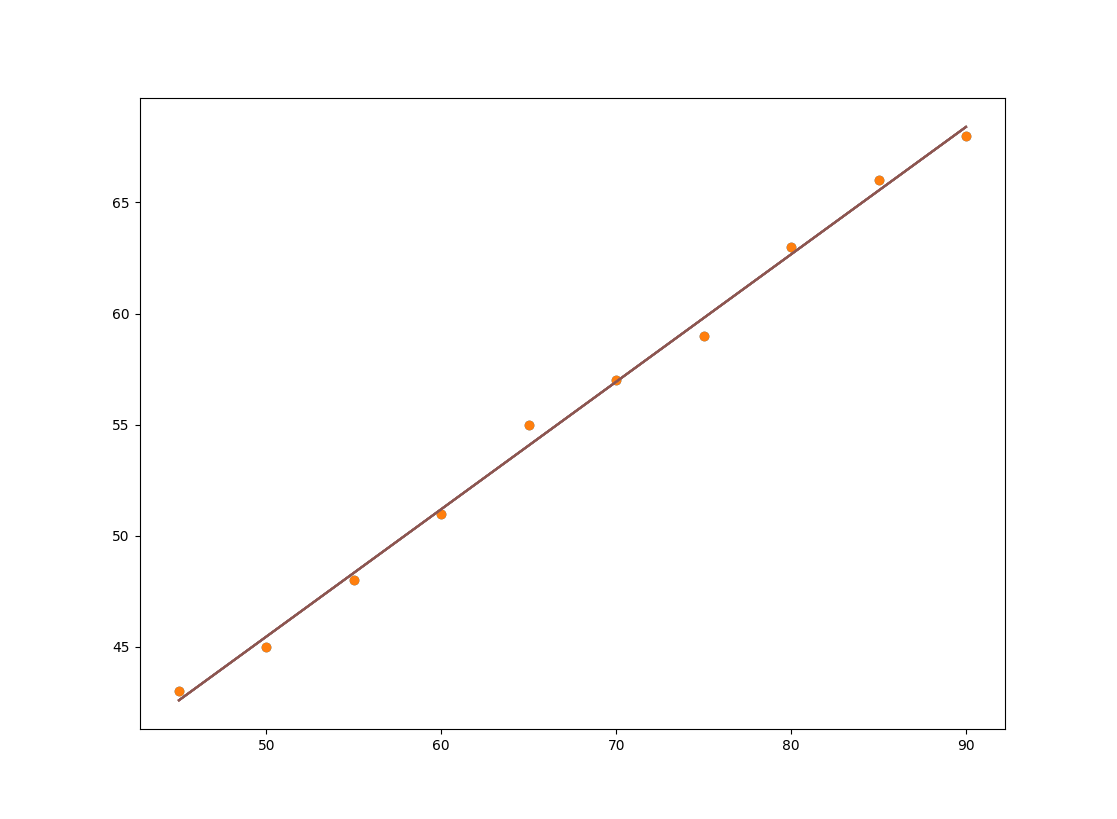
\includegraphics{img/reglin.png}
    }
    \\
    \textit{Représentation graphique obtenue avec Matplotlib}
\end{figure}
%
En orange sont affichés les points de $(x_i, y_i)$, et on voit plusieurs droites superposées de couleurs différentes, quasiment indiscernables : ce sont nos deux régressions linéaires ainsi que celle de Numpy (polyfit).
\\Les résultats sont donc concordants : visuellement, toutes les régressions linéaires donnent le même résultat sur ce jeu de donnée.
%
\\Les coeffcients sont de mêmes très proches voire égaux.

\subsection{Régression linéaire et descente de gradient}
L'algorithme utilisé est l'algorithme de gradient, afin d'estimer les paramètres de régression. L'idée ici est de voir la notion d'optimisation (cf. sujet).

\subsubsection{Descente de gradient}
La fonction qui effectue la descente de gradient est la fonction \textit{regression$\_$poly}, qui implémente l'algorithme.\\
Étant donné deux listes $x$ et $y$ de même taille, et avec comme autre paramètre $\lambda$ (le pas de descente), un paramètre initial $\beta^0$ et $\epsilon$ (la contrainte de précision), elle calcule la régression polynomiale en utilisant la méthode vectorielle (voir algorithme et formules sur le sujet).

\subsubsection{Résultats obtenus}
Malheureusement, notre solution est algorithmiquement correct mais il nous est impossible de retrouver des valeurs ne serait-ce qu'approchées des valeurs obtenues pour $\beta_0$ et $\beta_1$. Étant très sensible au paramètre $\lambda$, et étant donné qu'on ne disposait pas de méthode analytique pour le calculer (bien qu'il en existe une (ou plusieurs?)), le calcul par la fonction fonctionne dans le sens où il n'y a aucune erreur sur les calculs et sur la façon de les faire (d'où "algorithmiquement correct").\\
La comparaison que l'on peut faire par défaut est que le vecteur obtenu via la méthode du gradient (dans notre stricte cas) est extrêmement éloigné du vecteur obtenu par méthode de régression linéaire vectorielle.

\section{Étude et manipulation de lois de probabilités}
\subsection{Loi Binomiale}
Pour représenter graphiquement la loi de probabilité pour les trois donnés dans le sujet, et puis qu’ici on est dans le cas de la loi binomiale, c'est la fonction \textit{binom.pmf(k, n, p)} de la bibliothèque \texttt{scipy.stats} qui sera utilisée.\\
Pour les trois cas, on obtient le graphique suivant :\\

\begin{figure}[H]
    \centering
     \scalebox{.65}{
     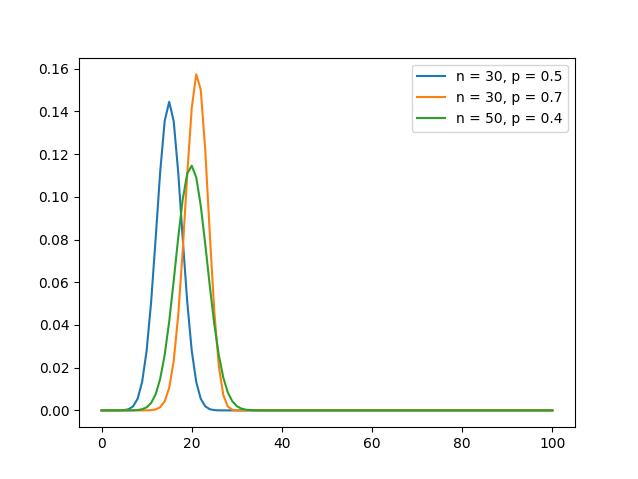
\includegraphics[scale=1]{img/loi_binomiale.png} 
    }
    \\
    \textit{Représentation de B(n, p) pour des valeurs de k $\in \llbracket 0, 100 \rrbracket$}
\end{figure}

On remarque que les courbes affichées ont une allure plutôt évidente de Gaussienne.

\subsection{Loi Normale univariée}

Pour représenter graphiquement la loi de probabilité pour les trois donnés dans le sujet, et puis qu’ici on est dans le cas de la loi binomiale, c'est la fonction \textit{norm.pdf(x, $\mu$, $\sigma$)} (fonction de densité de probabilités) de la bibliothèque \texttt{scipy.stats} qui sera utilisée.\\
Pour les trois cas, on obtient le graphique suivant :\\

\begin{figure}[H]
    \centering
     \scalebox{.65}{
     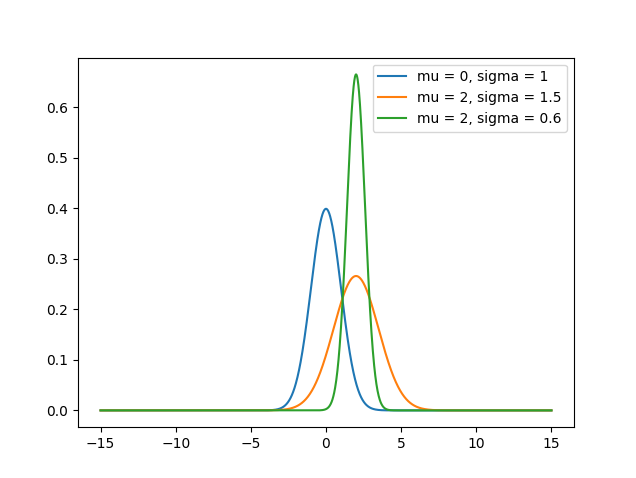
\includegraphics[scale=1]{img/loi_normale_univariee.png} 
    }
    \\
    \textit{Représentation de N($\mu$, $\sigma$) pour des valeurs de x $\in$ [-10, 10]}
\end{figure}

\subsection{Simulation de données à partir d’une loi}
Dans cette partie, on cherche à simuler des données à partir de la loi normale.\\
\subsubsection{Cas de la loi normale}

Dans la cas de la loi normale, on utilise la fonction \textit{tirage$\_$alea} afin de créer un échantillon de taille $n$ d'une loi normale centrée réduite (obtenue via la fonction \textit{normal($\mu$, $\sigma$, n) de la bibliothèque \texttt{numpy.random}}).\\
Les exécutions porterons sur des échantillons de taille 100, 1000, 10 000, 100 000 et 1 000 000.
Seront affichés sur chaque sous-graphique l'histogramme de l'échantillon et la fonction de densité de probabilité de la loi normale centrée réduite.\\
\begin{figure}[H]
	\centering
	\scalebox{0.35}{
	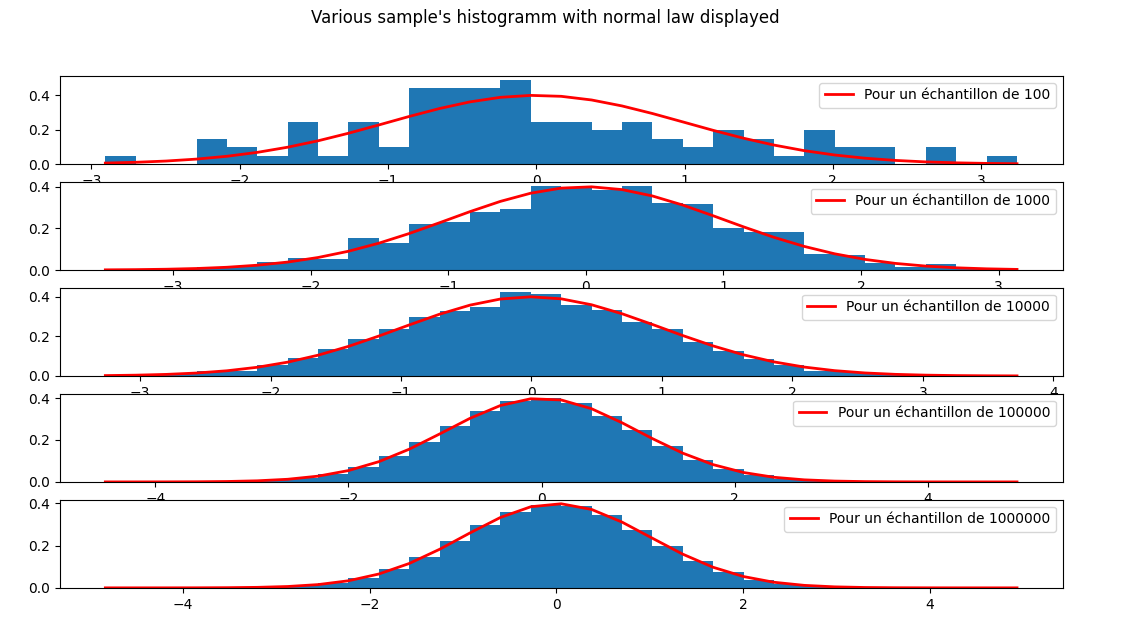
\includegraphics[scale=1]{img/estimation_loi_normale.png} 	
	}
	\\
	\textit{Échantillons de taille $n$ avec la densité de la loi normale centrée réduite}
\end{figure}

\subsection{Estimation de densité}
Dans cette partie, on cherche à estimer la densité pour différentes lois de probabilités.\\

\subsubsection{Cas de la loi normale}
Dasn le cas de la loi normale (plus précisément dans le cas de la loi normale centrée réduite), on génère un échantillon de taile $n$ selon la fonction \textit{tirage$\_$alea()} définie en partie \textbf{Simulation de données à partir d'une loi}, puis on estime $\mu$ et $\sigma$ grâce aux fonctions \textit{moyenne(..)} et \textit{ecart$\_$type(..)} (qui calculent ici la version empirique des paramètres) qui seront affichés dans le terminal et enfin on affiche la vraie densité (obtenue via la fonction \textit{normal(x, $\mu$, $\sigma$}) et la densité "estimée" afin de comparer les estimations.\\

\begin{figure}[H]
	\centering
	\scalebox{0.35}{
	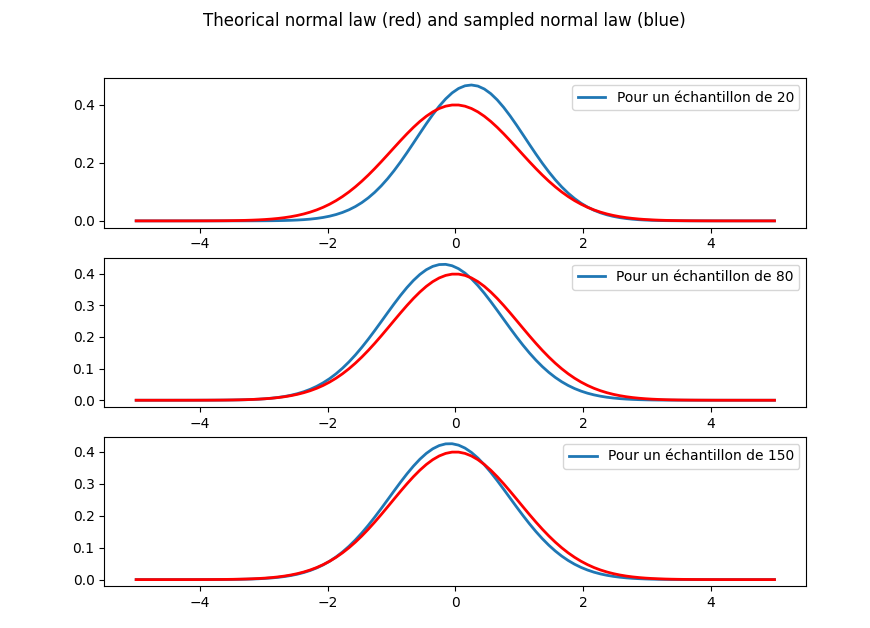
\includegraphics[scale=1]{img/estim_density_normale.png}  	
	}
	\\
	\textit{Comparaison entre la vraie densité et la densité avec $\mu$ et $\sigma$ estimés sur un  de taille $n$}
\end{figure}

On remarque que plus l'échantillon devient important,plus la densité "estimée" se resserre autour de la vraie densité (on remarque une sorte d'oscillation de la courbe autour du vraie $\mu$.\\


\subsubsection{Cas de la loi exponentielle}

\textbf{Pour la fonction de densité :}\\

De la même manière que pour l'estimation de la densité de la loi normale, on créé un échantillon de taille $n$ via la fonction \textit{echantillonage$\_$exp(..)} (utilisant la fonction \textit{exponential($\dfrac{1}{\lambda}$, $n$} de la bibliothèque \texttt{numpy.random}, qui revoit une valeur aléatoire de la densité exponentielle de paramètre $\lambda$), puis on estime et affiche $\lambda$ (grâce à la fonction \textit{estimation$\_$lambda(..)} où celle-ci utilise la fonction \textit{ecrat$\_$type(..)} (et donc moyenne) définie plus haut dans le code afin de réaliser l'estimation par MV. Enfin on représente la vraie densité (théorique) conjointement avec la densité empirique (estimée).\\

\begin{figure}[H]
	\centering
	\scalebox{0.35}{
	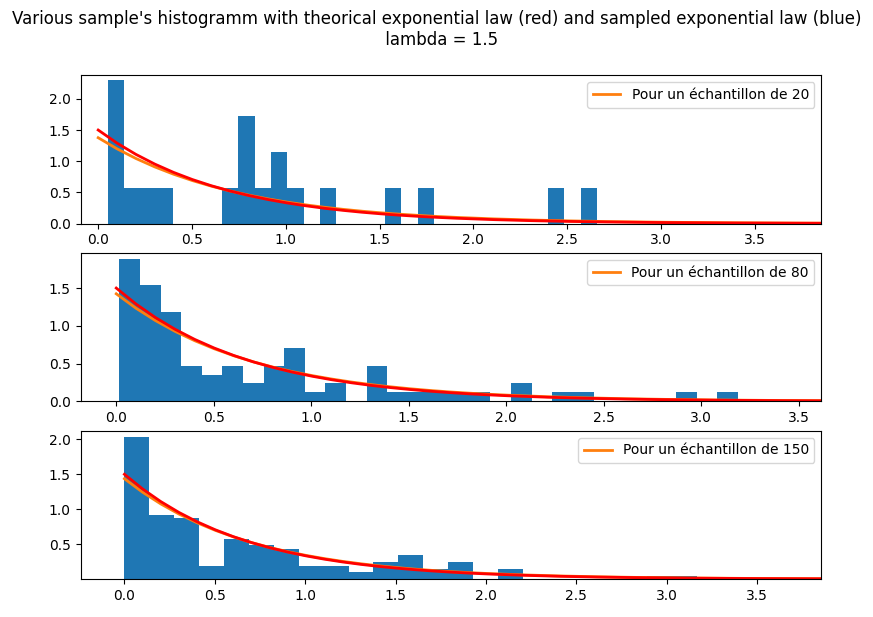
\includegraphics[scale=1]{img/estimation_densite_exponential.png}   	
	}
	\\
	\textit{Comparaison entre la vraie densité ($\lambda$ = 1.5) et la densité avec $\lambda$ estimé sur un échantillon de taille $n$}
\end{figure}

Conclusion : on remarque que l'estimation de $\lambda$ est d'autant plus précise à mesure que l’échantillon devient grand.\\
\newline
\textbf{Pour la fonction de répartition :}\\

On utilise la fonction d’échantillonnage pour la densité de la loi exponentielle (définie ci-dessus) et on estime $\lambda$. On sait que la fonction de répartition pour la loi exponentielle est : $$F(x) = \int_{-\infty}^{\infty} \lambda e^{-x\lambda}dx = 1 - e^{-x\lambda}$$.
Ainsi lors de l'affichage graphique, on calcule, sur les valeurs de l'échantillon, les valeurs de la fonction de répartition selon le vraie $\lambda$ et celui estimé.\\
On obtient le graphique suivant :\\

 \begin{figure}[H]
	\centering
	\scalebox{0.35}{
	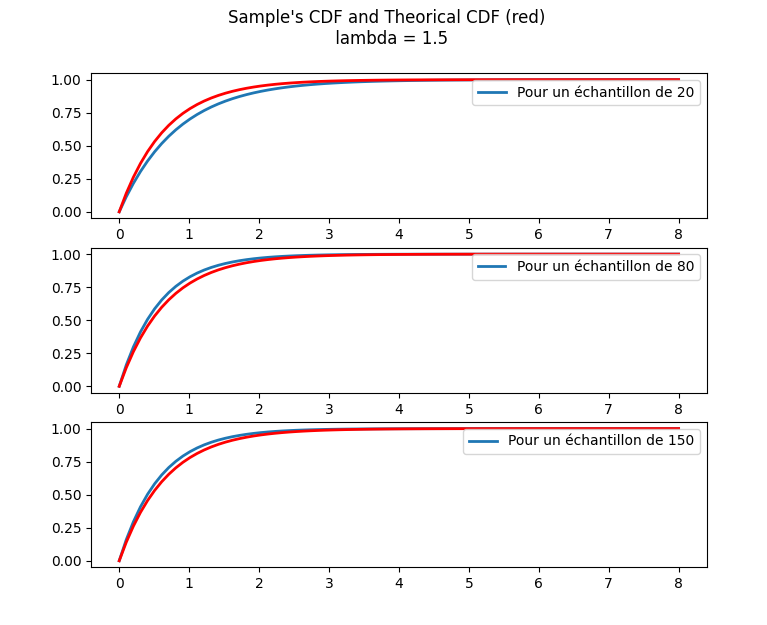
\includegraphics[scale=1]{img/cdf_expo.png}    	
	}
	\\
	\textit{Comparaison entre la vraie répartition ($\lambda$ = 1.5) et la répartition avec $\lambda$ estimé sur un échantillon de taille $n$}
\end{figure}

Sans surprise (étant donné qu'on utilise les mêmes fonctions d'obtention d’échantillon et d'estimation que dans le cas de la densité), puisque $\lambda$ est assez bien estimé, la répartition estimée "colle" de près la vraie répartition.

\section{Intervalles de confiance}
Le but de cette partie (correspondant au fichier \textsl{tp3.py}) est de déterminer les intervalles de confiances de différents échantillons statistiques afin de situer, selon une certaine précision, dans quelle plage de valeurs se situe l'espérance de l'échantillon.\\
Dans les 2 premiers problèmes, nous ne connaissons pas la variance de l'échantillon, ainsi la fonction calculant l'intervalle de confiance des échantillons utilisera la méthode de calcul via l'écart-type empirique et le fractile $t$ d'ordre $1-\dfrac{\alpha}{2}$ de la loi de student $St(n-1)$. Le problème 3, quant à lui, modélise un échantillon de taille $n$ de $B(p = \dfrac{1}{2})$. Ainsi la variance de la loi de Bernoulli est connue et vaut $p(1-p)$, donc dans ce cas là, le calcul de l'intervalle de confiance se fera via la formule utilisant l'écart-type véritable et \textit{u} le fractile d'ordre $1-\dfrac{\alpha}{2}$ de la loi $N(0,1)$.

\subsection{Fonctions}

La fonction \textit{intervalle$\_$confiance$\_$2} est utilisée dans le cas où on ne connaît pas la variance de notre échantillon (problème 1 et 2) alors que la fonction \textit{intervalle$\_$confiance$\_$1} est utilisée dans le cas où la variance de notre échantillon est connue (ou, dans les deux cas par ailleurs, la variance de la loi de la variable aléatoire constituant notre échantillon).
\textit{Voir les doc string Python pour les informations sur les fonctions, celles-ci donnent leurs rôles précisément}

\subsection{Problème 1}
On possède deux échantillons de taille 16 à notre disposition : un échantillon de masses de 16 pots de confitures mesurée en kilogramme (kg), et l'autre de masses d'avocats provenant du Mexique mesurée en grammes (g).\\

\textbf{$\rightarrow$On traite l'échantillon de masses en kg en premier.}\\

\textbf{Question 1 :} \\ La moyenne empirique obtenue est de 0.5 kg.\\
\textbf{Question 2 :} \\ L'histogramme obtenue sur l'échantillon des pots de confitures est le suivant\\

\begin{figure}[H]
    \centering
     \scalebox{.75}
     {
     	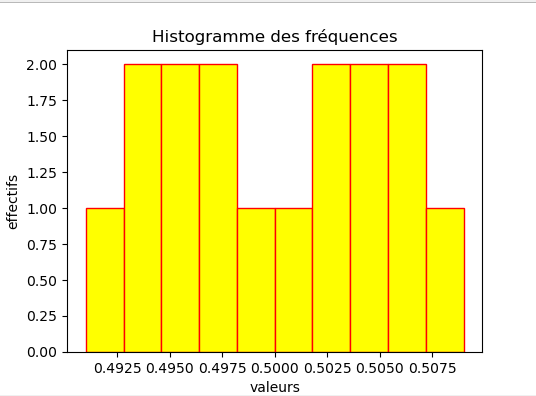
\includegraphics[scale=1]{img/histogr_frequ_masses_pots.png} 
     }
     \\
     \textit{Histogrammes des fréquences des masses des pots de confitures de l'échantillon}
\end{figure}

\textbf{Question 3 :} \\ On calcule les intervalles de confiances à 95$\%$ et à 99$\%$ pour l'échantillon des masses des pots. On obtient les intervalles suivantes : \\

\begin{center}
	\begin{itemize}
		\item $IC_{95\%}(\mu) = [0.497, 0.503]$
		\item $IC_{99\%}(\mu) = [0.496, 0.504]$
	\end{itemize}
\end{center} 

Il y a peu de différences dans notre cas entre l'intervalle à 95$\%$ et l'intervalle à 99$\%$. on remarque par ailleurs que pour une petite variation de l'ordre de $0.001$ sur chacune des bornes de l'intervalle de confiance à 95$\%$ pour passer à celle à 99$\%$, on obtient une variation de +0.04 sur la probabilité de trouver une masse dans celle-ci, (i.e $P(0.496 \le masse\_kg \le 0.504) = 0.99$) ce qui veut dire que la précision est affiné pour une très petite variation à cet ordre de sûreté.\\

$\rightarrow$\textbf{Quant à l'échantillon de masses des avocats du Mexique.}\\
Après calcul de son intervalle de confiance, avec toujours le fait que l'on ne connaisse pas sa variance, on obtient $IC_{95\%}(\mu) = [85.941, 88.558]$. Autrement dit, pour une masse en g d'un avocat de cet échantillon, on est sûr à 95$\%$ qu'il se situera dans cette intervalle, i.e $P(85.941 \le masse\_g \le 88.558) = 0.95$

\subsection{Problème 2}
Voici l'énoncé" du problème 2 : \textit{Une compagnie aérienne souhaite étudier le pourcentage de voyageurs satisfaits par ses services, on en a interrogé 500 choisis au hasard. Parmi eux, 95
se disent satisfaits. Déterminer un intervalle de confiance pour la proportion
inconnue de voyageurs satisfaits au niveau 99$\%$.}\\

On ne dispose pas d'échantillon mais on sait que $\dfrac{95}{500}$ personnes se disent satisfaites. On choisit ce même échantillon qui a été pris dans le cadre de l'énoncé (qu'on représente par une liste de 0 et de 1, 0 signifiant que la personne $i$ n'est pas satisfaite et 1 qu'elle est satisfaite) et on pose donc que la moyenne empirique vaut $\dfrac{95}{500}$. On en connait pas la variance de cet échantillon (étant donné qu'il ne suit pas une loi particulière, à priori). Ainsi, puisque la variance empirique est calculée lors de la détermination de l'intervalle de confiance, on exécute la fonction de calcul d'intervalle lors d'une non-connaissance de la variance.\\
On obtient l'intervalle suivant : $IC_{99\%}(\mu) = [0.145, 0.235]$ \\$\rightarrow$ i.e $P(0.145 \le proportion\_satisfaits \le 0.235) = 0.99$.\\

\textbf{Remarque :} on peut remarquer que la façon donc l'échantillon a été modéliser et les calculs faits que l'échantillon semble être un ensemble de 500 variables aléatoires suivant une loi de Bernoulli de paramètre $\theta$ compris dans notre intervalle de confiance.

\subsection{Problème 3}
Dans le problème 3, on utilise la fonction \textit{stats.bernoulli.rvs()} (fonctionnement détaillé dans \textbf{Fonctions}) qui nous permet de générer un tableau ( i.e un échantillon) de $n$ expériences de Bernoulli de paramètre $p = \dfrac{1}{2}$. On convertit ce tableau en liste pour travailler plus facilement dessus ( du fait que le tableau n'est qu'une dimension). Dans le cas présent, nous connaissons la variance, qui vaut très exactement $\sigma^{2} = p(1-p)$.\\
On calcule donc l'intervalle de confiance en prenant en compte ce fait (et donc en utilisant la fonction appropriée).\\
On obtient comme intervalles de confiance à 95$\%$ les intervalles suivants selon $n$ : \\

\begin{center}
	\begin{tabular}{|c|c|}
		\hline 
		$n$ & $IC_{95\%}(\mu)$ \\ 
		\hline 
		10 & $[0.19, 0.81]$ \\ 
		\hline 
		20 & $[0.331, 0.769]$ \\ 
		\hline 
		50 & $[0.381, 0.659]$ \\ 
		\hline 
		100 & $[0.422, 0.618]$ \\ 
		\hline 
		200 & $[0.501, 0.639]$ \\ 
		\hline 
		500 & $[0.428, 0.516]$ \\ 
		\hline 
		1000 & $[0.485, 0.547]$ \\ 
		\hline 
		10000 & $[0.49, 0.51]$ \\ 
		\hline 
		1000000 & $[0.498, 0.5]$ \\ 
		\hline 
	\end{tabular}
\end{center}

On remarque que plus l'effectif est grand, plus l'intervalle de confiance se réduit et devient précis quant à la valeur du paramètre trouvable à 95$\%$ dans celui-ci. 


\section{Exemples d'utilisation du code}
\subsection{Comment utiliser le code}
Concernant le code, il est séparé en trois fichier (comme dit plus haut en partie \textbf{\textit{Résumé de notre approche}}), chacun correspondant par son indice à la partie du TP correspondante (\textsl{tp$\_$3.py} avec la partie 3, \textsl{TP2.py} avec la partie 2, ...).
Si le code est exécuté sur l'IDE \texttt{Pyzo}, alors il est possible (après avoir exécuté "l'en-tête" du code, c'est à dire de la première ligne  au premier $\#\#$) d'exécuter séparément chaque sous partie du code, délimitées par \textit{$\#\#$ Problème x}.\\
Autrement, le code s'exécute normalement et en entier, si \texttt{Pyzo} n'est pas le logiciel où celui-ci est exécuté. Et bien penser à rentrer une valeur lorsque le programme le demandera (pour le problème 3 notamment).

\end{document}
